
%Contribution of Authors and Co-Authors Page
%\title{CHAPTER X \\ MICROBURST SCALE SIZE DERIVED FROM MULTIPLE BOUNCES OF A MICROBURST SIMULTANEOUSLY OBSERVED WITH THE FIREBIRD-II CUBESATS}

\chapter{CHAPTER FOUR \\ MICROBURST SIZE DISTRIBUTION DERIVED WITH AEROCUBE-6} \label{CH:ac6_study}

\section{Contribution of Authors and Co-Authors} 
\noindent Manuscript(s) in Chapter(s) 1 \\ 

\noindent Author: [type author name here] \\
Contributions: [list contributions here, single-spaced] \\
Co-Author: [type co-author name here] \\
Contributions: [list contributions here, single-spaced] \\
Co-Author: [type co-author name here] \\
Contributions: [list contributions here, single-spaced] \\

\iffalse
\authors{M. Shumko\affil{1}, A. Johnson\affil{1}, J. Sample\affil{1}, B.A. Griffith\affil{1}, D.L. Turner\affil{2}, T.P. O'Brien\affil{2},  J.B. Blake\affil{2}, O. Agapitov\affil{3}, S. G. Claudepierre\affil{2}}


\affiliation{1}{Department of Physics, Montana State University, Bozeman, Montana, USA}
\affiliation{2}{Space Science Applications Laboratory, The Aerospace Corportation, El Segundo, California, USA}
\affiliation{3}{Space Sciences Laboratory, University of California berkeley, Berkeley, California, USA}
\fi

\newpage




\section{Manuscript Information}

\noindent [Type Author and Co-author(s) Names Here] \\
Journal of Geophysical Research \\
Status of Manuscript: \textcolor{red}{Officially submitted to a peer-reviewed journal} \\
Wiley \\

\newpage

\section{Key Points}
\begin{itemize}
\item The dual AeroCube-6 CubeSats simultaneously observed $> 35$ keV microbursts at a variety of spatial separations ranging from $2$ to $\approx 100$ km.
\item In low Earth orbit the majority of microbursts have a size on the order of a few tens of km.
\item At the magnetic equator, the size of most microbursts corresponds to the size of whistler-mode chorus wave packets.
\end{itemize}

\section{Abstract}
Microbursts are an impulsive increase of electrons from the radiation belts into the atmosphere and have been directly observed in low Earth orbit and the upper atmosphere. Prior work has estimated that microbursts are capable of rapidly depleting the radiation belt electrons on the order of a day, hence their role to radiation belt electron losses must be considered. Losses due to microbursts are not well constrained, and more work is necessary to accurately quantify their contribution as a loss process. To address this question we present a statistical study of $> 35$ keV microburst sizes using the pair of AeroCube-6 CubeSats. The microburst size distribution in low Earth orbit and the magnetic equator was derived using both spacecraft. In low Earth orbit, the majority of microbursts were observed while the AeroCube-6 separation was less than a few tens of km, mostly in latitude. To account for the statistical effects of random microburst locations and sizes, a Monte Carlo and analytic models were developed to test hypothesized microburst size distributions. A family of microburst size distributions were tested and a Markov Chain Monte Carlo sampler was used to estimate the optimal distribution of the microburst size model parameters. Finally, a majority of observed microbursts map to sizes less then $200$ km at the magnetic equator. Since microburst are widely believed to be generated by scattering of radiation belt electrons by whistler mode waves, the observed microburst size correlates to coherent whistler mode chorus sizes derived in prior literature.

\section{Introduction}
Since the discovery of the Van Allen radiation belts in the 1960s by \citet{Allen1959} and \citet{Vernov1960}, decades of research has made headway in understanding the various particle acceleration and loss mechanisms. One of the extensively studied mechanisms responsible for both acceleration and loss is wave-particle scattering between whistler-mode chorus waves and electrons \citep{Abel1998_1, Meredith2002, Horne2003, Thorne2005, Millan2007, Bortnik2008}. Whistler-mode chorus waves are typically generated by a temperature anisotropy of low energy electrons up to tens of kiloelectronvolts (keV) and are typically found in the $\sim 0-12$ magnetic local times (MLT) \citep{Li2009, Li2009b}. Whistler-mode chorus waves interact with radiation belt electrons, and are widely believed to cause electron precipitation termed microbursts \citep[e.g.][]{Millan2007}.

Microbursts are a subsecond impulse of electrons that are observed by high altitude balloons and satellites in low Earth orbit (LEO) on radiation belt magnetic footprints $\sim 4 - 8$ L-shell (L) \citep[e.g.][]{Anderson1964, Lorentzen2001a, O'Brien2003, Tsurutani2013, Woodger2015, Crew2016, Breneman2017, Mozer2018, Greeley2019}, mostly in the dawn MLTs, and with an enhanced occurance rate during disturbed magnetospheric times \citep{O'Brien2003, Douma2017}. Microburst's role as a radiation belt electron loss mechanism has been estimated to be significant, with total radiation belt electron depletion due to microbursts estimated to be on the order of a day \citep{Lorentzen2001b, O'Brien2004, Thorne2005, Breneman2017}. These average microburst loss estimates are not well constrained due to assumptions made regarding the microburst precipitation region.

One of the unconstrained microburst parameters that is critical to better quantify the role of microbursts as an instantaneous loss mechanism (the number of electrons lost per microburst) is their physical size. Historically, after the bremsstrahlung X-ray signatures of microbursts were discovered by \citet{Anderson1964}, numerous microburst size studies were done using other balloon flights in the mid 1960s. \citet{Brown1965_2} used data from a pair of balloons separated by 150 km, mainly in longitude, and found that one third of all microbursts observed were temporally coincident. \citet{Trefall1966} then used the results from \citet{Brown1965_2} to model the probability that a microburst will be observed by two balloons as a function of the radius of the microburst, radius of the precipitating area a balloon is sensitive to, and the balloon separation. \citet{Trefall1966} concluded that the microbursts reported by  \citet{Brown1965_2} must have had a diameter of $230$ km assuming a balloon has a circular field of view with a $140$ km diameter (for electrons stopped at $100$ km altitudes). Soon after, \citet{Barcus1966} used a pair of balloons and concluded that a microburst must have a $<200$ km longitudinal extent. Then \citet{Parks1967} used data from a single balloon with four collimated scintillators oriented in different directions and found that the size of some mostly low energy microbursts to have a diameter of $80 \pm 28$ km, and others were less than $40$ km. 

Direct observations of microburst electrons are made by LEO spacecraft. \citet{Blake1996} found a microburst with a size of a few tens of km using the the Solar Anomalous and Magnetospheric Particle Explorer (SAMPEX) and concluded that typically microbursts are less than a few tens of electron gyroradii in size (order of a few km in LEO). Recently, \citet{Dietrich2010} used SAMPEX observations in another case study and concluded that the observed microbursts were smaller than $4$ km. \citet{Crew2016} used the Focused Investigation of Relativistic Electron Bursts: Intensity, Range, and Dynamics (FIREBIRD-II) CubeSats and found an example of a microburst larger than 11 km. Lastly, \citet{Shumko2018a} also used FIREBIRD-II to identify a microburst with a size greater than $ 51 \pm 1$ km. If anything, the large variance in prior results imply that there is a distribution of microburst scale sizes which this study aims to estimate.

Besides addressing the instantaneous radiation belt electron losses due to individual microbursts, the microburst size distribution is useful to identify the wave mode(s) responsible for scattering microbursts. By mapping the microburst size distribution in LEO to the magnetic equator it can be compared to the wave sizes estimated in prior literature. This comparison can be used to identify the waves and their properties (e.g. amplitude or coherence) responsible for scattering microburst electrons.

This paper addresses these two questions by expanding the prior microburst size case studies by analyzing microburst observations over a three year time period to estimate the microburst size distribution in LEO and the magnetic equator. The twin AeroCube-6 (AC6) CubeSats are utilized for this study because they were ideally equipped to observe microbursts simultaneously over a span of three years while their total separation varied between 2 and 800 km, mostly in latitude (in-track in orbit). This paper first describes the AC-6 mission, including their orbit and instrumentation in section \ref{instrumentation}. Section \ref{microburst_detection} develops the methodology used to identify microbursts observed by each spacecraft and how they were combined to make a list of simultaneously observed microbursts. Section \ref{microburst_distribution} describes the methodology used to estimate the microburst size distributions in LEO and the magnetic equator as a function of AC6 separation. Then a model is developed to shed light on how the compounding effects of a hypothesized microburst shape, size distribution, and random microburst locations will be observed by AC6, a two-point measurement platform. Lastly, in section \ref{discussion} we discuss these results and compare the microburst sizes estimated here to the size distribution of the whistler-mode chorus waves that are believed to cause microbursts. 

\section{Instrumentation} \label{instrumentation}
The AC6 mission consists of a pair of 0.5U (10x10x5 cm) CubeSats built by The Aerospace Corporation and launched on June 19th, 2014 into a 620 x 700 km, $98^\circ$ inclination orbit. The two satellites, designated as AC6-A and AC6-B, separated after launch and drifted apart. Both AC6 units have an active attitude control system which allows them to adjust the atmospheric drag experienced by each AC6 unit by orienting their solar panel ``wings" with respect to the ram direction. By changing their orientation, AC6 was able to achieve fine separation control and maintain a separation between 2-800 km. Figure \ref{fig1}a shows the AC6 separation for the duration of the mission. Figure \ref{fig1}b shows where AC6 was taking 10 Hz data simultaneously as a function of L and MLT which highlights that most data was taken at 8-12 MLT, an ideal local time for observing microbursts. Lastly Fig. \ref{fig1}b shows that the AC6 orbit was roughly dawn-dusk, sun-synchronous and precessed only a few hours in MLT over a three year period.

Each AC6 unit is equipped with three Aerospace microdosimeters (licensed to Teledyne Microelectronics, Inc). The dosimeter used for this study is dos1 and is identical on both AC6 units. Dos1 has a 35 keV electron threshold and all dosimeters sample at 1 Hz in survey mode, and 10 Hz in burst mode in the radiation belts. More detailed technical information on AC6 is described in \citet{O'brien2016}. 

\begin{figure}
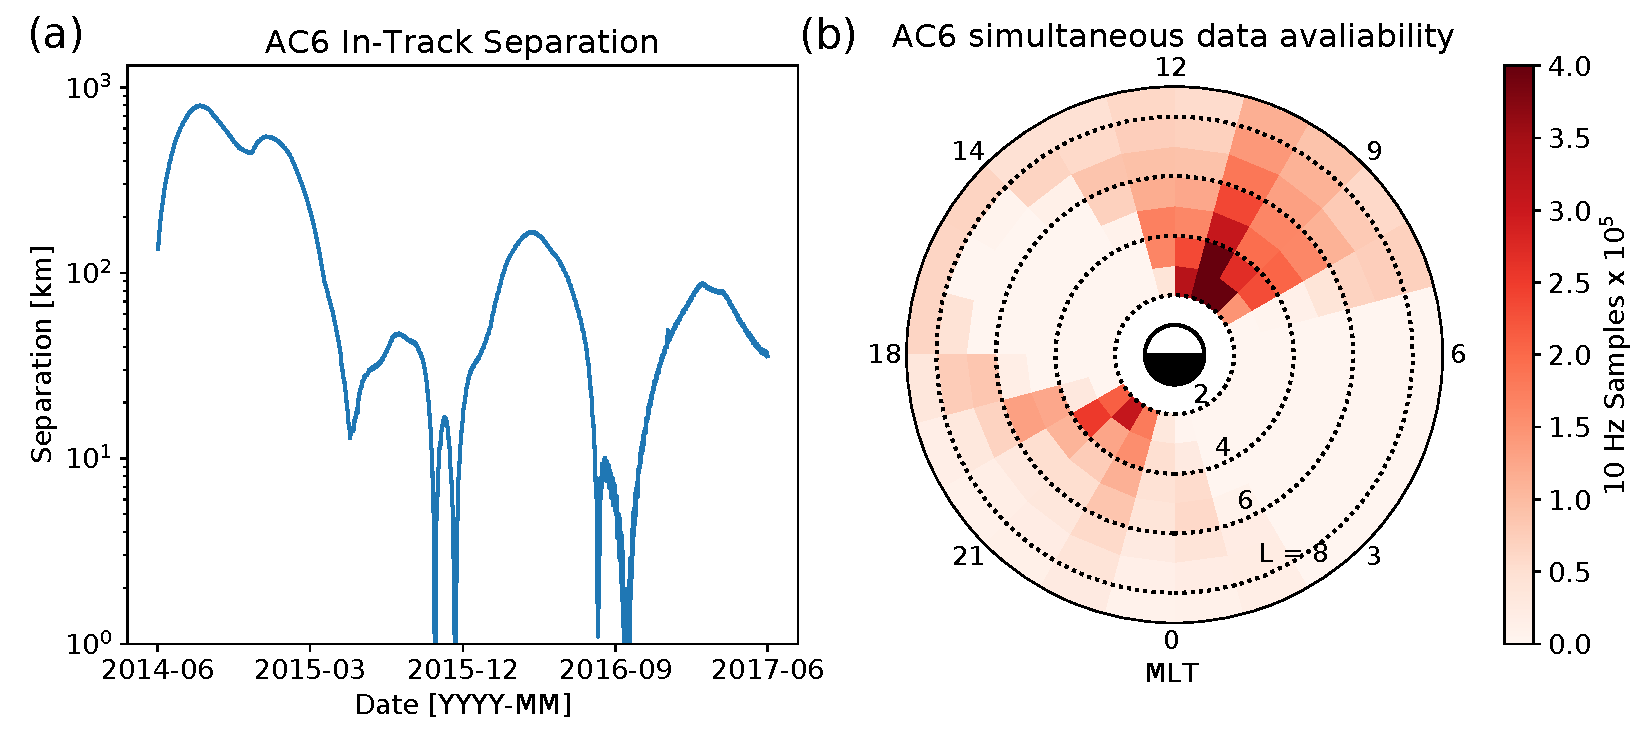
\includegraphics[width=\textwidth]{4_fig1.pdf}
\caption{AC6 mission properties for (a) spacecraft separation and (b) number of simultaneous quality 10 Hz samples as a function of L and MLT.} \label{fig1}
\end{figure}

\section{Methodology} 
\subsection{Microburst Detection} \label{microburst_detection}
The first step to find microbursts observed simultaneously by AC6 is to identify them on each individual spacecraft. Microbursts were detected with two different methods that yielded quantitatively similar results. The first method is the burst parameter \citep{O'Brien2003}. This algorithm has been successfully used in other microburst studies, mainly with the microbursts observed by SAMPEX \citep[e.g.][]{O'Brien2003, Blum2015, Douma2017}. For AC6, a burst parameter threshold of 5 was determined to be a good trade-off between false positive and false negative microburst detections. Another microburst detection algorithm based on wavelet spectra frequency filtering was developed and the resulting list of microbursts is similar to the list from the burst parameter.

With the two microburst detection lists in hand, data cleaning to remove microburst-like transmitter noise was necessary. The transmitters on AC6 can cause unphysical count impulses in the dosimeters that resembles periodic trains of microbursts. One source of transmitter noise was observed at times when AC6 was in contact with the ground stations above the US for data downloads and commanding, thus the microburst detections made above the US that were mostly at low L were discarded. 

Another source of noise is crosslink transmissions between AC6-A and AC6-B. These transmissions occurred when either spacecraft transitioned from the survey mode to 10 Hz mode. This noise is sometimes not caught by the data quality flag, so the following empirically-derived criteria were developed to remove those detections. The dosimeter with a 250 keV nominal electron threshold, dos2, was used because it had a nearly identical response to noise while rarely responded to microbursts. Since the transmitter noise is very periodic with a $\approx 0.2$ s period, cross-correlation (CC) and autocorrelation (AC) methods were applied to the dos1 and dos2 time series. Detections were discarded if the following two criteria were met: either dos1 or dos2 time series had a AC peak at a $0.2$ or $0.4$ s lag and the dos1-dos2 CC was greater than 0.9. The AC lag criteria alone sometimes falsely removed legitimate trains of microbursts, so the second criteria insured that the detection was removed if there was also an unphysically high correlation across an order of magnitude in energy.

The lists of microbursts observed individually by AC6 were then merged into a list of temporally correlated microbursts, i.e. microbursts that were observed simultaneously by both AC6 units, with the following procedure. The general idea is that a microburst detected by one spacecraft will cross-correlate well with the time series from the other spacecraft if it observed a similar microburst, and poorly if there was no microburst observed by the other spacecraft. Each microburst detection made by either spacecraft was cross-correlated with the time series from the other spacecraft whether or not a microburst was observed by the other spacecraft. Cross-correlation windows with 1 and 1.2 s widths were chosen with slightly different window sizes to account for random count variation due to Poisson noise. Microbursts detections that had a cross-correlation greater than $0.8$ were considered temporally coincident. This CC threshold was chosen as it is low enough to accept user-identified temporally coincident microbursts superposed with noise, and high enough to reject most non-coincident events. Figure \ref{fig2}, panels (a), (c), (e), and (g) show examples of microbursts observed by both AC6 units when they were separated by 5, 16, 37, and 69 km, respectively. 

The last criteria requires that the temporal CC must be greater than the spatial CC + 0.3. The spatial CC was calculated by shifting one spacecraft's time series by the in-track lag to cross-correlate in the same spatial location, i.e. latitude. This criteria was applied to remove curtains, stationary structures observed by AC6 that are narrow in latitude \citep{Blake2016} that can be misidentified as microbursts. Figure \ref{fig2}, panels (b), (d), (f), and (h) show the shifted time series to confirm that there were no spatially correlated, non-microburst structures present. Lastly the merged microburst list was spot checked by two authors to remove poorly correlated and any duplicate events. After filtering out transmitter noise and applying the CC criteria, 662 simultaneous microburst detections were found and used in this study.

\begin{figure}
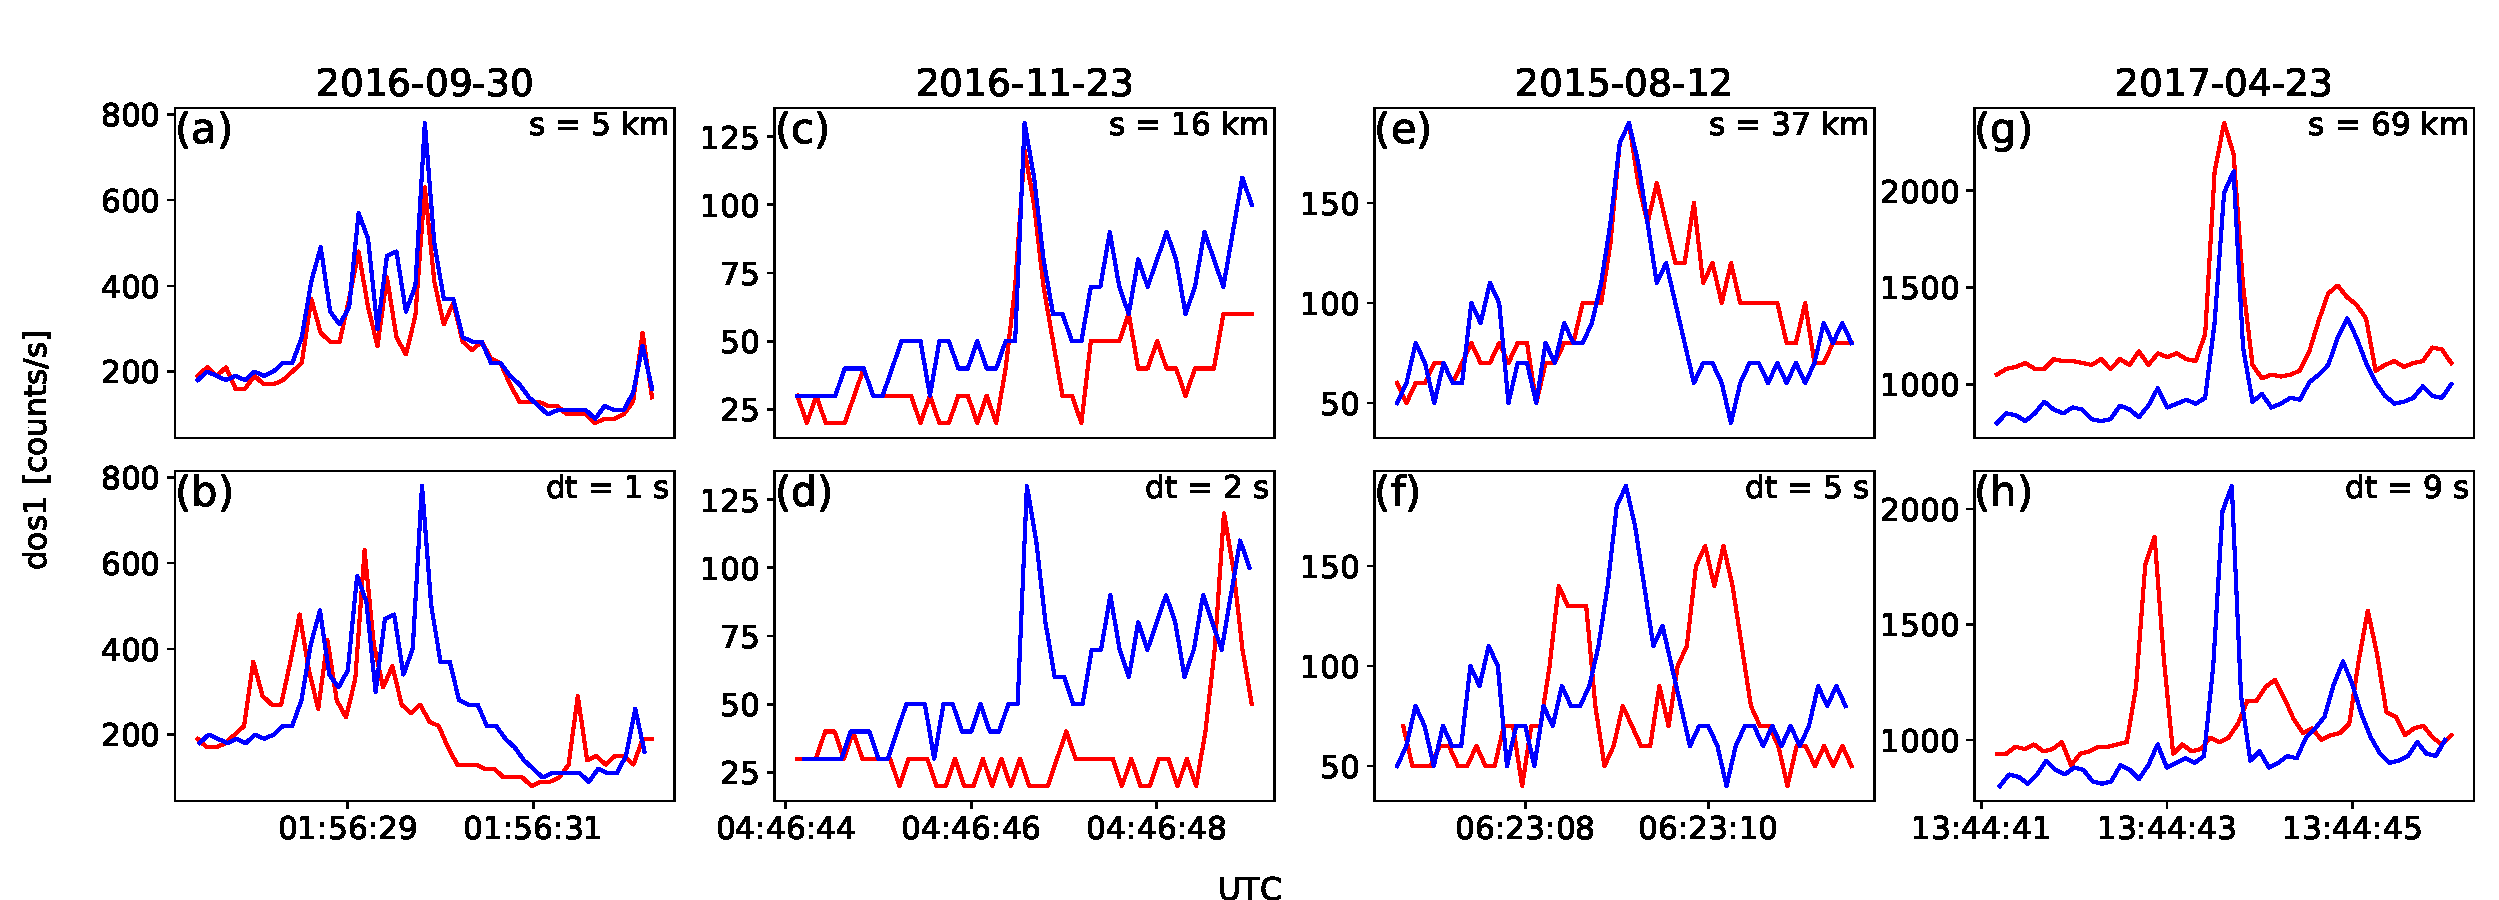
\includegraphics[width=\textwidth]{4_fig2.pdf}
\caption{Examples of $>35$ keV microbursts observed simultaneously by AC6-A in red and AC6-B in blue. Panels (a), (c), (e), and (g) show the temporally-aligned time series when AC6 were separated by $s=$ 5, 16, 37, and 69 km, respectively. The corresponding panels (b), (d), (f), and (h) show the spatially-aligned time series which is made by shifting the AC6-A time series in the above panels by the in-track lag (annotated with $dt$) that show any spatially correlated structures. The clear temporal correlation and lack of spatial correlation demonstrates that these events are microbursts.} 
\label{fig2}
\end{figure}
	

\subsection{Microburst Size Distribution in LEO and Magnetic Equator}\label{microburst_distribution}
The temporally coincident microbursts, which from now on will be referred to as microbursts, are now used to estimate the fraction of microbursts observed above AC6 separation, $s$. When AC6 observes a microburst at $s$, the microburst's size must be greater than $s$. This fact, along with the arguments presented in Section 4 in \citet{Joy2002} who studied the most probable Jovian magnetopause and bow shock stand off distances, are used to investigate the dependence of the number of microbursts observed above $s$, as a function of $s$. This dependence is the microburst complementary cumulative distribution function $\bar{F}(s)$. 

The cumulative fraction of microbursts observed above $s$ is the ratio of $N(s)$, the normalized number of microbursts observed above $s$, to $N(0)$, the total number of microbursts observed 
\begin{equation}
\bar{F}(s) = \frac{N(s)}{N(0)}
\end{equation} where N(s) is defined by

\begin{equation}
N(s) = \sum_{i = s}^\infty n_{i} \Big( \frac{S_{max}}{S_{i}} \Big)
\end{equation} where $n_{i}$ is the number of microbursts observed by AC6 in ith separation bin. The normalization term $S_{max}/S_{i}$ is a ratio of the number of 10 Hz samples in the most sampled separation bin to the number of samples in the ith bin. This normalization factor corrects AC6's non-uniform sampling in separation, thus $\bar{F}(s)$ can be interpreted as the fraction of microbursts observed above $s$ assuming AC6 sampled evenly in separation. Microburst $\bar{F}(s)$ in LEO is shown by the black curve in Fig. \ref{fig3}a for $4 < \mathrm{L}< 8$ and split into one L-wide bins with the colored curves. The separation bin width used in Fig. \ref{fig3} is 5 km. To check for bias in $\bar{F}(s)$ due to the choice of separation bins, $\bar{F}(s)$ was resampled using other bin widths and offsets. Bin widths as large as $20-30$ km and bin offsets did not qualitatively effect the curves in Fig. \ref{fig3}a. The normalization i.e., the number of 10 Hz samples in each separation bin, is shown in \ref{fig3}c.

The overall trend in Fig. \ref{fig3}a shows a sudden cumulative probability drop off, followed by a shoulder up to $s \approx 70$ km where $\bar{F}(s)$ drops to nearly zero. A large negative gradient of $\bar{F}(s)$ at some separation implies that microbursts must be smaller than that separation. To quantify this, Fig. \ref{fig3}b shows the microburst probability density function (PDF), calculated by differentiating $\bar{F}(s)$. The microburst PDF shows a peak at $s < 30$ km as well as a peak between $70-80$ km separation. These PDF peaks are evidence of a sub $30$ km microburst population and larger microbursts observed up $70-80$ km separations. The shaded region around the black curves in Fig. \ref{fig3}a-b shows the standard error due to counting statistics. The uncertainty due to false coincidence events i.e. two unrelated microbursts lining up in time by random chance was also considered. The microburst duty cycle in a one minute window ($\approx 1 \ L$) around each microburst was calculated. The false coincidence probability is the square of the duty cycle and was found to be less than 5\% for the majority of microbursts. The false coincidence probability for each microburst was then used to randomly remove microbursts and $\bar{F}(s)$ was recalculated in $10^4$ trials. The spread in the $\bar{F}(s)$ trial curves with microbursts randomly removed was much smaller than the uncertainty due to counting statistics alone.

To compare the microburst size to the size of their hypothesized progenitor waves, the spacecraft locations during observed microbursts were mapped to the magnetic equator using the Olson-Pfitzer magnetic field model \citep{Olson1982} which is implemented with a Python wrapper for IRBEM-Lib \citep{irbem}. As previously stated, a microburst observed in LEO has a size larger than the spacecraft separation, hence that microburst would also have a size larger than the spacecraft separation after it was mapped to the magnetic equator. Thus the procedure to estimate $\bar{F}(s)$ is identical to the LEO size distribution but with a different normalization. The normalization factors were calculated by mapping every quality AC6 sample to the magnetic equator and binning them by equatorial separation into 100 km wide bins. Figure \ref{fig4} shows the equatorial microburst size distribution in the same format as Fig. \ref{fig3}. The equatorial PDF trend is similar to LEO and most of the microbursts were observed when the AC6 equatorial separation was less than 200 km. 

The results in Figs. \ref{fig3} and \ref{fig4} show the fraction of microbursts observed above a spacecraft separation and do not fully represent the microbursts size distribution due to the compounding effects from the range of microburst sizes and random locations of microbursts with respect to AC6 i.e. even if the microburst size is much larger than the AC6 separation, some fraction of those microbursts will be only observed by one AC6 spacecraft. Thus modeling is necessary to capture the compounding influence of these statistical effects on AC6.

\begin{figure}
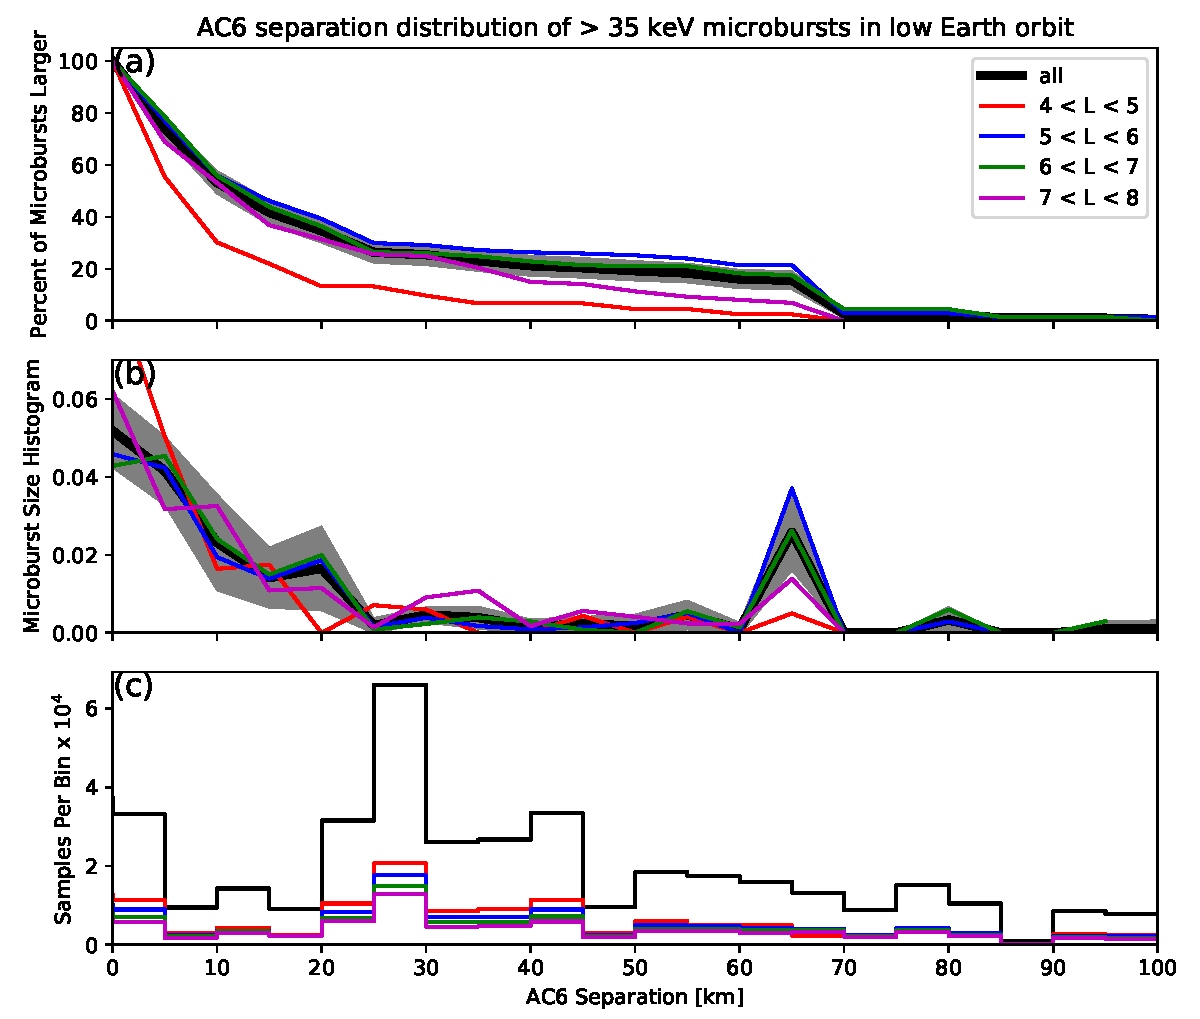
\includegraphics[width=\textwidth]{4_fig3.pdf}
\caption{Microburst size distribution in low Earth orbit. Panel (a) shows the percent of microbursts observed above that separation after normalizing for the uneven AC6 sampling in separation. Panel (b) shows the microburst probability density (size histogram) as a function of separation. Lastly, panel (c) shows the normalization, i.e. number of simultaneous samples AC6 observed as a function of separation. The colored lines show the distributions binned by L, and the thick black curve for the entire radiation belt ($4 < L < 8$). The gray shading around the black curve shows the uncertainty due to counting statistics.}
\label{fig3}
\end{figure}

\begin{figure}
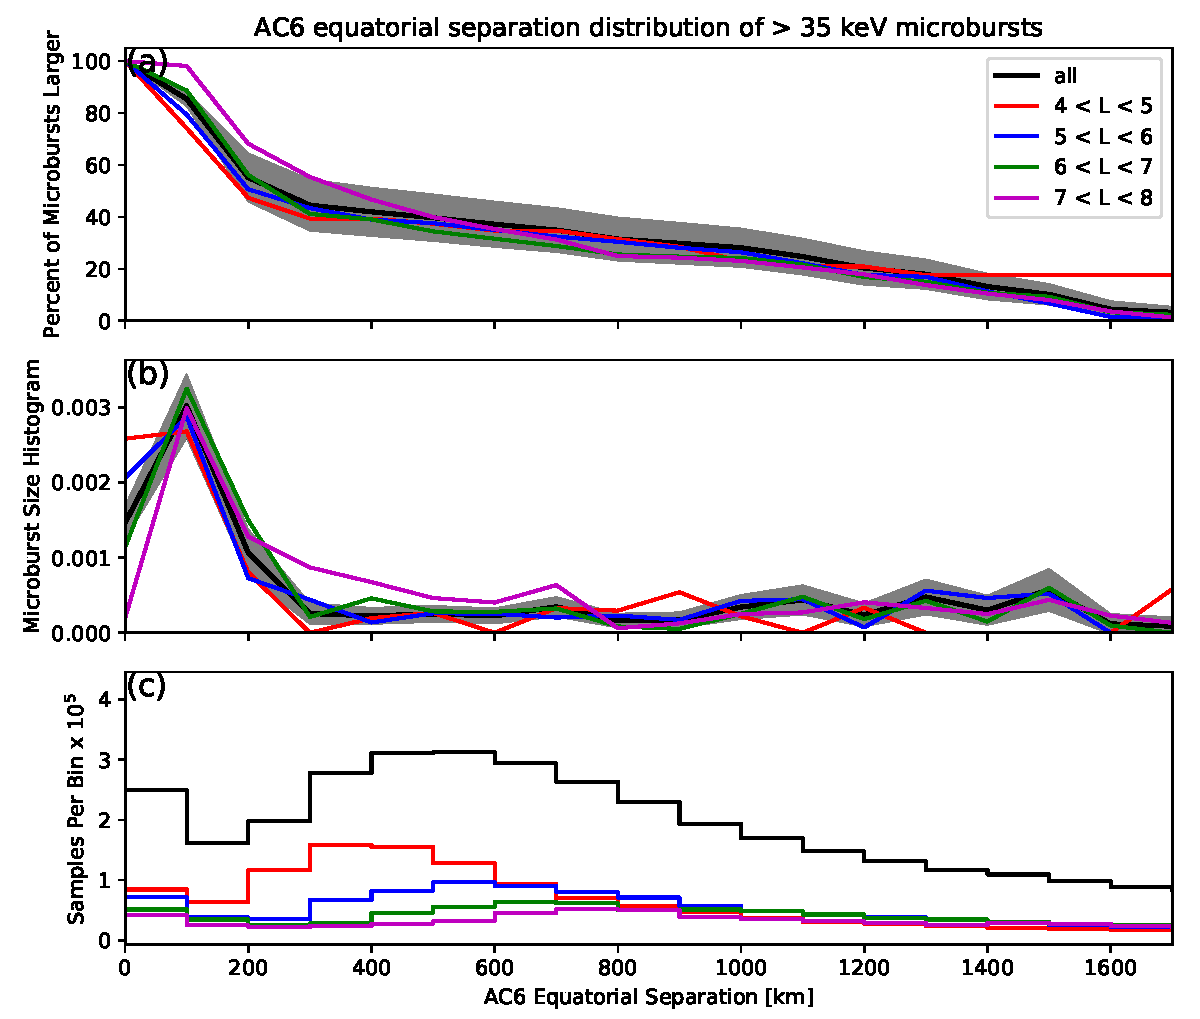
\includegraphics[width=\textwidth]{4_fig4.pdf}
\caption{Microburst size distribution mapped to the magnetic equator in the same format as Fig. \ref{fig3}.} 
\label{fig4}
\end{figure}

\section{Modeling the Distribution of Microburst Sizes} \label{model_section}
\subsection{Monte Carlo and Analytic Models to Calculate $\bar{F}(s)$}

To account for the effects due to microbursts randomly occurring around AC6 with an unknown distribution of microburst sizes, Monte Carlo (MC) and analytic models were developed. These models assume a hypothesized distribution of microburst sizes expressed with a probability density function $p(d | \theta)$ where $\theta$ are the dependent variables, and a microburst footprint shape to estimate $\bar{F}(s)$. The microburst footprint is assumed to be circular with a diameter $d$. $p(d | \theta)$ can be understood as ``the probability of observing a microburst of diameter $d$, given the parameters $\theta$''. Various microburst size distributions were considered: a one-size and two-size microburst populations, and continuous $p(d | \theta)$ such as Maxwell, Weibull, and log-normal.

The Monte Carlo model is the most intuitive. It first randomly scatters $10^5$ microburst centers in a 400 x 400 km grid around AC6. Then each microburst center was assigned a diameter, randomly picked from a $p(d | \theta)$ distribution after $\theta$ parameters were specified. Spacecraft A is placed at the origin, and spacecraft B is placed along the positive y-axis at distances from spacecraft A corresponding to the AC6 separation bins used in Section \ref{microburst_distribution}. Then for each spacecraft B location, the number of microbursts that encompass both spacecraft was counted. The modeled fraction of microbursts observed above $s$ is then

\begin{equation}
\bar{F}(s) = \frac{\displaystyle\sum_{i > s}^\infty n_{i} }{ \displaystyle\sum_{i > 0}^\infty n_{i} }.
\end{equation} where as before the number of microbursts observed by both spacecraft in the ith bin is $n_{i}$.

The analytic model, while identical to the MC model, highlights the geometrical concepts connecting $p(d | \theta)$ and $\bar{F}(s)$ with geometry arguments similar to \citet{Trefall1966}. For a microburst with $d = 2r \geq s$, there is an area between AC6 where that microburst will be observed by both spacecraft if the microburst's center lands there. Figure \ref{fig5}a-c shows this geometry with the two spacecraft indicated with black dots with varying relations between $r$ and $s$. All microbursts who's center lies inside the circular area of radius $r$ surrounding either spacecraft will be observed by that spacecraft. If it exists, the intersection of the two circular areas around both spacecraft defines another area, $A(r, s)$ where a microburst will be observed by both spacecraft if the microburst center lands there. This area can be calculated using the circle-circle intersection area equation, 
\begin{equation}
A(r, s) = 2r^2 \cos^{-1}{\Big( \frac{s}{2r} \Big)} - \frac{s}{2} \sqrt{4r^2 - s^2}.
\end{equation} Example geometries where $A(r, s) > 0$ are shown in Fig. \ref{fig5}b and c. With this conceptual model and $A(r, s)$, the analytic form of $\bar{F}(s)$ can be found and is derived in the Supporting Information (SI) Text S1. To demonstrate the effects of random microburst locations near AC6, examples of the analytic and Monte Carlo $\bar{F}(s)$ curves are shown in Fig. \ref{fig5}d for a one-size, $d=40$ km microburst population.

\begin{figure}
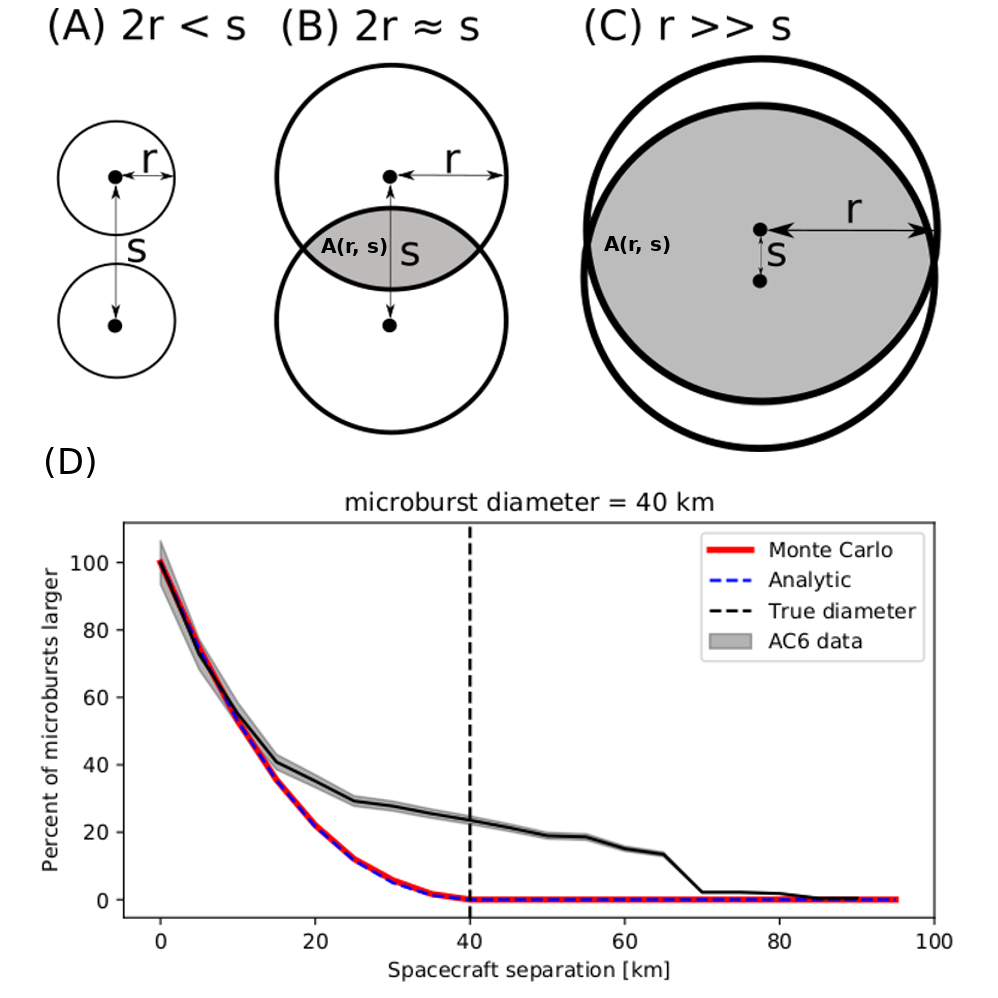
\includegraphics[width=\textwidth]{4_fig5.png}
\caption{Panels A-C show the varying geometries of the analytic model. The two spacecraft are shown as black dots. The enclosing black circle around each spacecraft bounds the area where a microburst will be observed by one or both AC6 units if the microburst's center lies inside the circle. Panel (A) shows the case where microburst diameter is smaller than the AC6 separation and all microbursts will be observed by either unit A or B and never simultaneously. Panel (B) shows the intermediate case where the microburst diameter is comparable to the AC6 separation and some fraction of microbursts will be observed simultaneously. The fraction of the microbursts simultaneously observed is proportional to the circle intersection area $A(r, s)$ and is shown with grey shading. Panel (C) shows the case where the microburst diameter is much larger than the spacecraft separation and nearly all microbursts will be observed by both spacecraft. Lastly panel (D) shows $\bar{F}(s)$ from the AC6 data with a solid black line, and modeled MC and analytic $\bar{F}(s)$ curves for a single-sized microburst distribution with $d = 40$ km.} 
\label{fig5}
\end{figure}

\subsection{Methods for estimating optimal $\theta$ parameters}
At this stage we have all of the ingredients to calculate $\bar{F}(s)$ given a prescribed $p(d | \theta)$. For each $p(d | \theta)$ tested, the optimal $\theta$ parameters are estimated in this study using the traditional least squares regression and Bayesian inference. While we report the $\theta$ parameters that minimize least squares, this section focuses on Bayesian inference because it seamlessly incorporates statistical uncertainty in the data. The uncertainty in the data is then propagated to $\theta$ which is then no longer an optimal value, rather a distribution of values that is consistent with the observations and its uncertainty. 

Bayesian inference is rooted in Bayes theorem of conditional probability. Given the observed $\bar{F}(s)$ as $y$, and model's dependent variables as $\theta$, Bayes theorem can be written as

\begin{equation}
p(\theta | y) = \frac{p(y | \theta) p(\theta)}{p(y)}.
\end{equation} $p(\theta)$ is the distribution of $\theta$ that describe our prior level of knowledge about that parameter e.g. from earlier microburst size studies, a microburst size must less than $500$ km in LEO. This is called the prior which is quantified by a PDF such as normal, uniform, etc. Next term is the likelihood, $p(y | \theta)$, the conditional probability of obtaining $y$ given a particular $\theta$. The likelihood probability is a probabilistic penalty function that quantifies the discrepancy between the modeled and observed $\bar{F}(s)$ in terms of the standard error. The resulting PDF of $\theta$s consistent with the observations is $p(\theta | y)$ known as the posterior distribution. The posterior is an update to our prior distributions, modified by the likelihood i.e. the data and its uncertainties. Here, the posterior is used to make inferences regarding the range of $\theta$ parameters that generate a $\bar{F}(s)$ that is consistent with the observations. The last parameter in Bayes theorem is $p(y)$. $p(y)$ is the marginal likelihood (evidence) that describes the probability of obtaining $y$ after marginalizing over all prior variables. Calculation of $p(y)$ is difficult, and often not necessary for model parameter estimation. 

With all of the above terminology, the important takeaway is that the posterior distribution for each model parameter is interpreted as the range of our model's dependent parameters that are consistent with the observations. A 95\% credible interval (CI) for each model parameter is reported here that is interpreted as: assuming a hypothesized $p(d | \theta)$, there is a 95\% probability that the true $\theta$ is inside the CI. To sample the posterior distribution, the $\theta$ parameter space is explored with a Markov Chain Monte Carlo (MCMC) sampler. In a nutshell a Markov Chain is a process that samples random variables that depend on only the previous state of those random variables. Hence a MCMC sampler is a Monte Carlo sampler that samples the $\theta$ parameter space by picking random $\theta$ values based on the previous state of $\theta$. 

The first and one of the most popular MCMC is the Metropolis-Hastings sampler \citep{Metropolis1953, Hastings1970}. While the Metropolis-Hastings sampler is explained in detail in \citet{Metropolis1953} and \citet{Hastings1970} and a good introduction given in \citet{Sambridge2006} as well as \citet{Sharma2017}, a brief overview is warranted. The Metropolis-Hastings sampler samples the posterior distribution in $N$ trials. Once an initial set of $\theta$ is randomly picked from the prior, the i$^{th}$ trial involves the following steps. First calculate the posterior probability for $\theta_i$. Then pick a proposal $\theta_{i+1}$ to jump to, randomly picked near $\theta_i$ in parameter space. If the $\theta_{i+1}$ posterior probability is higher than $\theta_i$, the MCMC accepts the proposal and moves to $\theta_{i+1}$. If the posterior probability of $\theta_{i+1}$ is smaller than $\theta_{i}$, there is a random chance that $\theta_{i+1}$ will be accepted or rejected (if rejected, $\theta_{i+1} = \theta_i$ and a new proposal is generated). This accept/reject criteria allows the sampler to trend to more probable $\theta$ while also exploring the neighboring regions. After the $N$ trials, a histogram is made using the accepted $\theta$s to produce the posterior distribution for each model parameter.


\subsection{Estimating optimal parameters for various microburst size models}
The MCMC sampler is first used to test the simplest microburst size model where all microbursts are one size and the MCMC will estimate that size. The microburst size PDF for this model can be expressed as
\begin{equation}
p(d | d_0) = \delta(d-d_0)
\end{equation} where $\delta$ is the Dirac Delta function and $d_0$ is the diameter of all microbursts according to this model. The range of $d$ that are consistent with the observed $\bar{F}(s)$ is shown in Fig. \ref{fig6}. Assuming this model, there is a $95 \%$ probability that the microburst diameter is between 38 and 129 km. As a sanity check the optimal size that minimizes least squares is 73 km.

A slight generalization of the one-size model is a two-size microburst population model that assumes the following microburst PDF
\begin{equation}
p(d | d_0, d_1, a) = a \delta(d-d_0) + (1-a)\delta(d-d_1)
\end{equation} where the diameters of the two microburst populations are given by $d_0$ and $d_1$ and $a$ is the parameter that quantifies the relative fractions of the two populations. The result of this model is shown in Fig. \ref{fig7}. The fit is slightly better than the one-size model, although that is to be expected given two more free model parameters. A majority, $98$ \%, of microbursts, have a diameter between $12$ and $47$ km with a rare population with a diameter between $76$ and $234$ km. The set of parameters that minimize least squares is $99.5$ \% of microbursts are small with a size of $21$ km and the remaining $0.5$ \% of microbursts have a $140$ km size.

Other, continuous PDFs were tested including: Maxwellian (Maxwell -- Boltzmann), log-normal, and Weibull. The range of model parameters that are consistent with the observed $\bar{F}(s)$ are presented in the SI text S2. These distributions were chosen because they have the following properties that are most realistic: they are continuous, approach 0 in the limit as $r \rightarrow 0$ (lower bound microburst size is ultimately limited by the electron gyroradius), and can be symmetrical or asymmetrical.

\begin{figure}
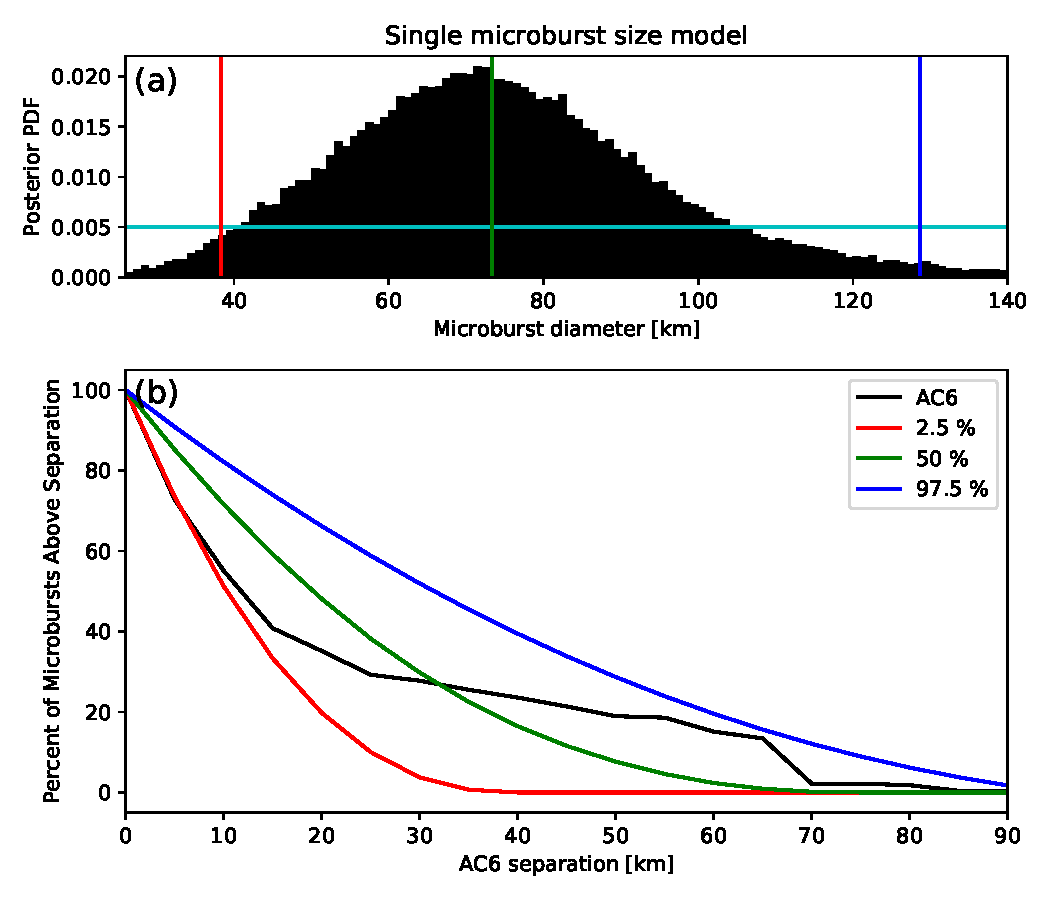
\includegraphics[width=\textwidth]{4_fig6.pdf}
\caption{Range of plausible microburst sizes assuming all microbursts are one fixed size. Panel (a) shows the posterior probability density function of microburst diameters in black. The red, green, and blue vertical lines at 38, 73, and 129 km represent the 2.5, 50, and 97.5 posterior percentiles, respectively. A uniform prior between 0 and 200 km was assumed for this MCMC run and is shown in cyan. Panel (b) shows the percent of microbursts observed above an AC6 separation for $4 < L < 8$ in black. The 2.5, 50 and 97.5 size percentiles were estimated from the posterior and plotted in red, green, and blue curves, respectively.} 
\label{fig6}
\end{figure}

\begin{figure}
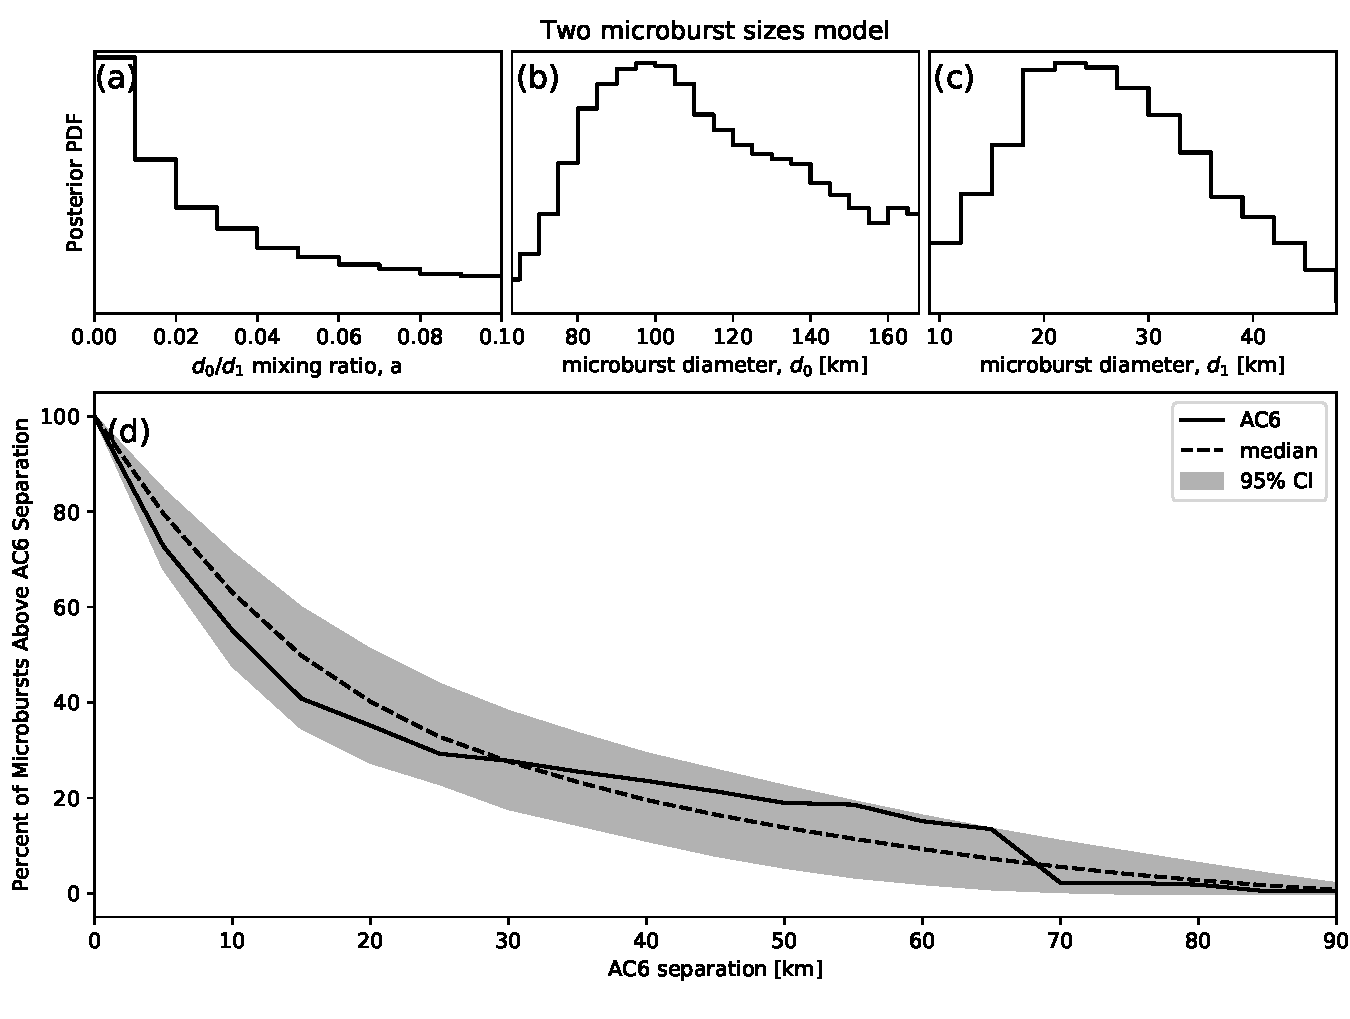
\includegraphics[width=\textwidth]{4_fig7.pdf}
\caption{Plausible microburst percent curves assuming microburst size distribution is bimodal consisting of two sizes $d_0$ and $d_1$ with a mixing term that quantifies the relative occurrence of the $d_0$ to $d_1$ microburst populations. Panel (a) shows the posterior distribution for the microburst population mixing term, $a$ with a median value of $0.02$. The $a$ prior was uniform between 0 and 0.2. Panel (b) shows the posterior distribution for $d_0$, the larger microburst population estimated with a uniform prior between 50 and 200 km and the posterior median diameter of $122$ km. Panel (c) shows the posterior distribution for $d_1$, the smaller microburst population, estimated using a uniform prior between 0 and 50 km with a median diameter of $28$ km. Panel (d) is similar to Fig. \ref{fig6}b and shows the AC6 microburst fraction for $4 < L < 8$ in black. A set of 1000 random parameter triples ($a$, $d_0$, and $d_1$) were drawn from the posterior and used to generate a family of $\bar{F}(s)$ curves. At each $s$ the range of consistent $\bar{F}(s)$ were quantified by the 2.5, 50 and 97.5 percentiles and shown with the red, green, and blue curves, respectively.} 
\label{fig7}
\end{figure}

\section{Discussion} \label{discussion}
The LEO microburst $\bar{F}(s)$ estimated in section \ref{microburst_distribution} shows that a majority of coincident microbursts were observed by AC6 when they were separated by less than a few tens of km. This conclusion is consistent with prior literature and most similar to \citet{Parks1967} who reported that many $> 15$ keV microbursts are less than $40$ km in diameter while others were on average $80 \pm 28$ km in diameter. Furthermore, these results are similar to the bouncing packet example shown in \citet{Blake1996} with a size of ``at least a few tens of kilometers". The relatively small number of large $> 70$ km microbursts observed by AC6 fit in well with the results from \citet{Barcus1966} and \citet{Brown1965_2}, although the AC6 separation is mostly latitudinal while \citet{Barcus1966} and \citet{Brown1965_2} used data from pairs of balloons separated predominantly in longitude. 

Without knowledge of the microburst shape, a direct comparison between the AC6 and balloon observations is difficult. \citet{Trefall1966} discussed how a hypothetical circular microburst at the scattering location near the magnetic equator will be stretched into an ellipse with a semi-major axis in the longitudinal direction. This stretching effect should be explored further as it introduces an ambiguity from the eccentricity of the ellipse that prevents a direct latitudinal and longitudinal comparison.

When comparing our results to more recent studies, the AC6 microburst size distribution is much larger than the sizes reported in \citet{Dietrich2010} who used very low (VLF) frequency transmission paths and SAMPEX to conclude that microbursts must be smaller than 4 km from a small number of microbursts observed during one SAMPEX radiation belt pass. \citet{Dietrich2010} arrived at their conclusion by looking for temporal coincidence of microbursts and FAST events, subsecond VLF transmission perturbations, but the connection between FAST events and microbursts is not well understood. Lastly, our results are consistent with FIREBIRD-II observations of a $> 11$ km microburst reported by \citet{Crew2016}, and the minority of microbursts observed by AC6 up to $s \approx 70$ km are consistent with the $> 51$ km bouncing packet microburst reported in \citet{Shumko2018a}.

The microburst PDF shown in Fig. \ref{fig3}b suggests that the microburst size distribution is bimodal. This has been suggested before by \citet{Blake1996} who noted that the $> 150$ keV and $> 1$ MeV microbursts are not always well correlated e.g. Fig. 10 in \citet{Blake1996}. The quality of the AC6 data is insufficient to definitively conclude that there are two distinct microburst populations. The different microburst population hypothesis can be better tested with an AC6-like mission with better energy resolution and homogeneous MLT coverage.

The model results from section \ref{model_section} emphasize that care must be taken when comparing the $\bar{F}(s)$ curves observed by AC6 and the true microburst size distribution due to the compounding effect of an unknown microburst size distribution, unknown microburst shape, and random microburst locations near AC6. By assuming there is only one microburst size, the results in Fig. \ref{fig6} suggest that there is a 95\% probability that the microburst diameter is somewhere between 38 and 129 km, a relatively wide range of values. On the other hand, the two-size model has a smaller variance around the AC6 $\bar{F}(s)$, which is expected with the addition of two more free parameters. The two size model is interpreted as 98\% of microbursts diameters are between 12 and 47 km and larger microbursts are very uncommon. 

A variety of continuous $p(d)$ such as the Maxwellian, Weibull and log-normal were also tested. While the continuous microburst PDFs are more realistic, there is no clear choice of which microburst PDF nature prefers. The one and two-size model are simple to interpret, and the two-size model qualitatively fits the observations the best out of all $p(d)$ tested. Surely nature does not only have two discrete microburst sizes. Rather, the current evidence and reasoning supports a bimodal and continuous PDF hypothesis. Due to lack of prior observations and theoretical predictions, it is difficult to identify and test a more appropriate $p(d)$ hypothesis at this time.

The equatorial microburst $\bar{F}(s)$ estimated in section \ref{microburst_distribution} and Fig. \ref{fig4}b in particular shows that the majority of microbursts were observed when the equatorial AC6 separation was less than $200$ km. We will now explore how these results compare to prior multi-point measurements of chorus source sizes made near the magnetic equator. The International Sun-Earth Explorers (ISEE 1 and 2) were used by \citet{Gurnett1979} to make one of the first direct chorus source scale measurements. \citet{Gurnett1979} estimated that the wave power correlation scale was on the order of a few hundred km across the background magnetic field. Using the Cluster Wide Band Data measurements \citet{Santolik2003} found the correlation scale of whistler mode chorus waves to be around 100 km near the source region at $L \approx 4$ and midnight MLT sector. Furthermore, \citet{Turner2017} used the four satellites comprising the Magnetospheric Multiscale Mission and found that rising tone whistler mode chorus elements were phase coherent up to 70 km at $L \approx 8$. Lastly, \citet{Agapitov2010, Agapitov2011b, Agapitov2017a, Agapitov2018} used multiple sets of spacecraft missions with wave measurements near the chorus source region to statistically show that the extent of chorus source region can extend from 600 km in the outer radiation belt to greater than 1,000 km in the outer magnetosphere.

The equatorial microburst size of less than a few hundred km shows that the waves responsible for scattering microburst electrons must have correlated properties on those scales. The wave properties necessary for scattering microburst electrons e.g. coherence, polarization, wave normal angle, etc. can be identified by studying the waves properties that are only observed by multiple equatorial spacecraft at small separations. These properties can then aid wave-particle scattering model development by constraining the wave properties and scattering modes responsible for scattering microburst electrons. In turn, future models could then make predictions regarding the distribution of microburst sizes in LEO. 

\section{Conclusions}
In conclusion, the twin AC6 CubeSats enabled the detailed statistical study of microburst sizes from a two point measurement platform. Roughly $60 \%$ of the $> 35$ keV microbursts were simultaneously observed while AC6 was separated by less than $20$ km and the rest were observed up to $\approx 70$ km separation. Modeling the microburst cumulative distribution function is essential to quantify the relationship between the number of microbursts observed as a function of separation to a hypothesized microburst size distributions. The AC6 microburst data, together with modeling, has hinted at the existence of a bimodal microburst size PDF with the majority of microbursts with a diameter smaller than $40$ km and a rare microburst population with a diameter around $100$ km. The bimodal size hypothesis may be more comprehensively addressed from LEO spacecraft with more simultaneous microburst observations, homogeneous MLT coverage, and differential energy channels. Moreover, to disentangle the compounding effect that affects two-point microburst measurements, a X-ray imager on a high altitude balloon can observe the atmospheric microburst footprint and determine the microburst size, shape, and any spatial correlations with little ambiguity. 

When mapped to the magnetic equator, most microbursts were observed while the mapped AC6 separation was less than $200$ km. This correlates well with the sizes of highly correlated chorus waves and it suggests that the wave properties crucial for scattering microbursts must be correlated over relatively small regions. By studying the wave properties that are correlated on a few hundred km scales, the dominant wave scattering modes may be identified.

\section{Acknowledgments}
This work was made possible with the help from the many engineers and scientists at The Aerospace Corporation who designed, built, and operated AC6. M. Shumko was supported by NASA Headquarters under the NASA Earth and Space Science Fellowship Program - Grant 80NSSC18K1204. D.L. Turner is thankful for support from the Van Allen Probes mission and a NASA grant (Prime award number: 80NSSC19K0280). \textcolor{red}{Other Aerospace and MSU funding sources...} The AC6 data is available at http://rbspgway.jhuapl.edu/ac6 and the IRBEM-Lib version used for this analysis can be downloaded from https://sourceforge.net/p/irbem/code/616/tree/.